
%%% Local Variables:
%%% mode: latex
%%% TeX-master: t
%%% End:

\chapter{PARD原型系统实现与验证}
\label{chap:impl}

%FPGA原型设计目标
上一章已经讨论过如何在X86平台上实现PARD,本章讨论如何在gem5全系统模拟器上将PARD机制
实现其中。验证功能可行性,


\section{基础系统选择}

实现PARD原型系统的第一个工作是选择一个合适的基础系统,
PARD对基础系统有以下需求:

\begin{enumerate}
  \item 能够在FPGA环境下综合;
  \item 独立系统,不依靠任何辅助设施即可运行;
  \item 丰富的I/O设备支持,支持Xilinx VC709开发板所提供的外设,如以太网和PCI-Express;
  \item 能够运行Linux操作系统;
  \item 频率/性能足够运行常见Benchmark应用,如SpecCPU、PARSEC等);
  \item 可以运行典型的数据中心应用,如memcached、httpd等;
  \item 具备完整的软件开发环境;
\end{enumerate}

虽然在开源领域有大量可用的处理器软核,如Oracle OpenSPARC T1\cite{sparct1}、
RISC-V\cite{riscv}、OpenRISC\cite{or1k}、LEON3\cite{leon3}等,
但这些软核并不能满足PARD原型系统的需求。
其中OpenSPARC T1和RISC-V目前的FPGA实现并不是一个独立系统,
需要额外的处理器(如MicroBlaze或ARM)作代理以实现访存与I/O操作;
OpenRISC 1200的软件开发环境支持并不完整;
LEON3是目前开源的处理器软核中最为合适的选择,但其对linux内核的支持并不好,
目前只能运行早期的内核版本,同时软件环境也比较老旧,运行数据中心应用存在一定的困难。
一些FPGA厂商也提供了可配置的处理器核,
如Xilinx的MicroBlaze\cite{microblaze}和ARM\cite{zynq},以及Altera的NIOS II\cite{niosii}。

本文最终选择了Xilinx的MicroBlaze作为基础系统,
其处理器采用32位小端RISC架构,实现了单发射5级流水,
支持MMU及虚拟内存,使用AXI4作为外部总线接口\cite{microblaze-ref}。
该处理器软核在Virtex-7型号的FPGA上频率最高能够达到246MHz,
性能是354DMIPs(1.44DMIPs/MHz)\cite{microblaze},能够满足PARD原型系统的需求。

\begin{figure}[tb]
  \centering
  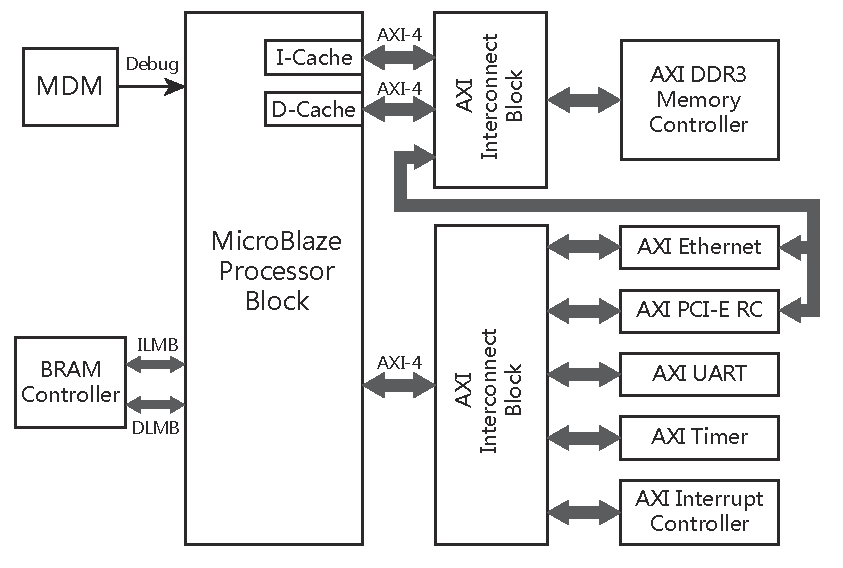
\includegraphics[width=0.6\textwidth]{impl/microblaze-base-arch}
  \caption{MicroBlaze基础架构}
  \label{fig:microblaze-base-arch}
\end{figure}


基于MicroBlaze的一个典型系统架构如图\ref{fig:microblaze-base-arch}所示,
MicroBlaze系统的固件代码保存在Block Memory中,
通过LMB(Local Memory Bus)总线连接到处理器核;
缓存子系统采用哈佛结构,具有分离的指令与数据缓存,它们通过AXI4总线连接到内存控制器;
I/O子系统同样使用AXI4总线互连,其中包括基本的外设,如中断控制器、串口、时钟等,
也支持一些复杂的I/O设备,如以太网\cite{axi-ethernet-subsystem}、
PCI-E\cite{axi-pcie-bridge}等。
MicroBlaze同时还提供了硬件调试接口,可以通过JTAG对其进行调试。

目前Xilinx提供的MicroBlaze软核并不支持多处理器架构,
在硬件实现上没有提供处理器间同步、通信机制,
之前一些工作\cite{microblaze-mp-rsp08,microblaze-mp-xapp}尝试为其增加多处理器支持,
但这些工作只是实现也最底层的处理器间同步、通信机制,
没有可用的操作系统层次上的多核支持。
受到该因素的影响,本文所设计的PARD原型系统只实现了``伪多核''的系统,
即系统中存在多个处理器核,但每个一逻辑域都被限制为只能使用一个处理器核。
未来MicroBlaze的多核软硬件支持完善后,可以很容易的将PARD原型系统的这一限制解除,
实现真正的多核系统。


\section{PARD原型系统}

PARD原型系统架构如图\ref{fig:pard-arch-impl}所示,
该系统由处理器子系统、I/O子系统、PRM SoC三部分组成。
其中处理器子系统包含四个处理器核心、共享缓存和内存控制器;
I/O子系统中包含四个串口控制器、两个以太网控制器和一个PCI Express根逻辑(RootComplex),
系统中所有的数据通路使用AXI4总线连接;
PRM同样是基于MicroBlaze的SoC系统,对外提供串口与SFP以太网接口,
同时通过内部串口与I/O子系统相连,用于接收I/O子系统的串口输出,
使用I2C总线作为控制平面网络的数据链路层,连接到系统中的四个控制平面:
处理器核控制平面CoreCP、共享缓存控制平面CacheCP、内存控制器控制平面MemCP和
I/O子系统控制平面I/OCP。

\begin{figure}[tb]
  \centering
  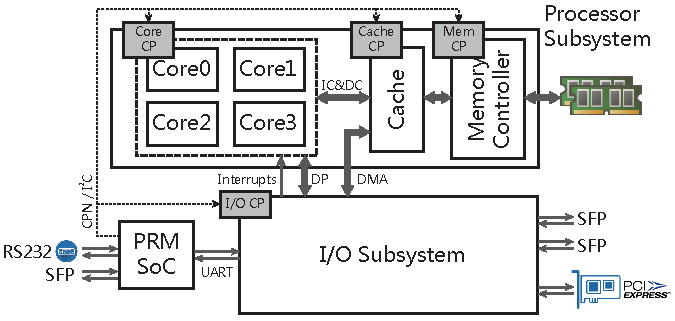
\includegraphics[width=0.8\textwidth]{impl/pard-arch-impl}
  \caption{PARD原型系统架构}
  \label{fig:pard-arch-impl}
\end{figure}

% 如何增加标签寄存器
处理器核心使用MicroBlaze软核及其它附属模块组成,
其内部结构如图\ref{fig:pard-core-impl}所示,
其中包含MicroBlaze软核、中断控制器和时钟模块,
该模块从外部输入时钟、复位和中断信号,
通过三个AXI4接口(IC指令缓存端口、DC数据缓存端口和DP外设端口)与外部交换数据。
AXI4总线协议中使用独立的通道实现读写请求、数据与响应,
其中读写请求中包含用户自定义信号,本文使用该信号在系统中传播应用标签。
由于MicroBlaze并没有开放源代码,处理器核的请求标记工作需要在核外进行:
首先在核外增加了一个标签寄存器,CoreCP连接到该寄存器,并可以对其内容进行修改;
在IC/DC/DP三个端口外分别增加三个标签模块,
用于将标签寄存器的值附加到AXI4总线AR/AW两个通道的USER信号中,完成请求标记。

% 增加共享缓存模块:支持16路、实现标签传播、实现划分
Xilinx为AXI4总线提供了一个缓存功能的IP核SystemCache\cite{pg118-system-cache},
其默认配置最多只能够支持4路组关联,这对于四核的PARD原型系统来说,
不足以验证缓存容量划分的功能,本文通过修改IP核实现,将其扩展到16路组关联;
按照第\ref{chap:labeladdrspace:propagation}节所述的方式,为该模块增加了标签传播功能;
同时修改其默认LRU替换策略,使其支持按路划分功能,
并通过CacheCP对共享缓存的行为进行控制(参见第\ref{chap:impl:cachecp}节)。
% 实现的多核
该Cache模块提供MicroBlaze专用接口连接四个处理器核,
同时还提供了通用AXI Master接口连接I/O子系统的DMA通道。
内存控制器控制平面提供了地址映射功能,实现四个处理器核的内存资源划分,
第\ref{chap:impl:migcp}节将详细讨论内存控制器控制平面的实现。

% I/O子系统结构
PARD的I/O子系统内部结构如图\ref{fig:pard-io-impl}所示,
处理器子系统的DP端口经过I/O子系统控制平面的地址映射后,使用AXI总线连接到所有的硬件模块,
其中PCI-E和以太网模块中包含DMA功能,
因此按照第\ref{chap:labeladdrspace:tagging}节中所描述的方法在其中增加标签寄存器,
其DMA访存请求结构标记后通过AXI总线发送到Cache模块。
所有设备的中断信号在内部进行编码,经过I/O控制平面进行重映射处理后,发送给对应的处理器核。
I/O子系统控制平面的设计将在第\ref{chap:impl:iocp}节进行讨论。

\begin{figure}[b]
\begin{minipage}{0.48\textwidth}
  \centering
  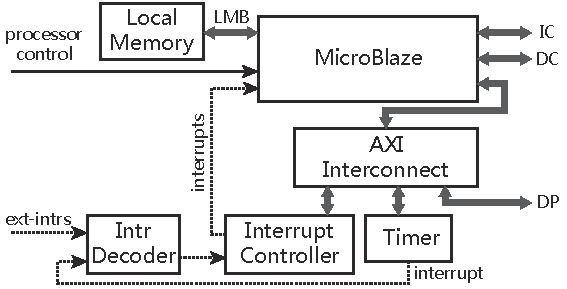
\includegraphics[width=\textwidth]{impl/pard-core-impl}
  \caption{PARD原型系统处理器核}
  \label{fig:pard-core-impl}
\end{minipage}\hfill
\begin{minipage}{0.48\textwidth}
  \centering
  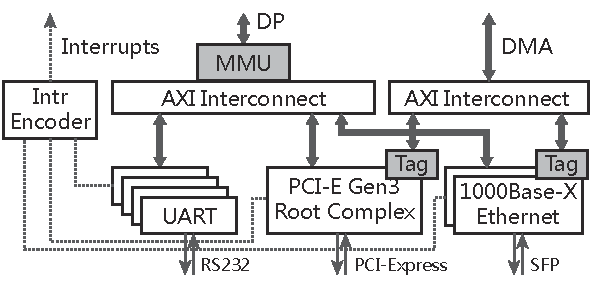
\includegraphics[width=\textwidth]{impl/pard-io-impl}
  \caption{PARD原型系统I/O子系统}
  \label{fig:pard-io-impl}
\end{minipage}
\end{figure}

% 原型的照片
本文使用Xilinx Virtex-7 FPGA(型号xc7vx690tffg1761-2)
在VC709平台上实现了上述PARD原型系统,如图\ref{fig:pard-fpga-board}所示。
该原型系统对外呈现三类接口:一个RS232串口,与PRM的串口相连;
三个SFP接口,其中两个连接到I/O子系统,另外一个与PRM的以太网接口相连;
一个PCI-E Gen3 x4接口,连接到I/O子系统,可以连接兼容的PCI-E设备,
在本例中在该接口连接了一块Intel PCI-E以太网卡(芯片型号82575)。

\begin{figure}[tb]
  \centering
  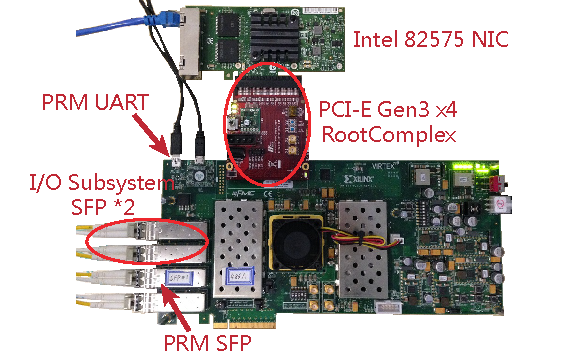
\includegraphics[width=0.6\textwidth]{impl/pard-fpga-board}
  \caption{PARD原型系统}
  \label{fig:pard-fpga-board}
\end{figure}

% 资源占用与FPGA布线结果
该原型系统在FPGA上的布局布线结果如图\ref{fig:pard-fpga-routed}所示。

% TODO: 增加资源使用情况,以及分模块的资源占用情况




\section{PRM与软件栈实现}

为何选择I2C,有何替代

如何改造I2C成为双向网络

连接多个控制平台

触发表中断传播机制
在第\ref{chap:impl:trigger-latency}节中将对触发表响应时间进行分析。


LDom的内核、rootfs和device-tree(完整的)


\section{控制平面实现}

\subsection{通用控制平面}

\subsubsection*{表设计}
\subsubsection*{状态表更新逻辑}
\subsubsection*{触发表逻辑}


\subsection{处理器核控制平面}
\label{chap:impl:corecp}

\subsection{共享末级缓存控制平面}
\label{chap:impl:cachecp}


\textbf{延迟分析}\quad
We find that the LLC control plane does not introduce
extra latency. According to Figure 4, the processing logic of the
LLC control plane can be hidden into the pipeline of the LLC
controller. In fact, pipelining is a typical design for modern CPUs’
LLC. For example, the L2 cache of OpenSPARC T1 has eight
pipeline stages, our Xilinx Cache has five stage pipeline.
Furthermore, synthesis data verify that the logic
of the LLC control plane is not in critical pathes.


\subsection{内存控制器控制平面}
\label{chap:impl:migcp}

\textbf{延迟分析}\quad
为实现内存控制器平面地址映射功能,在数据通路的关键路径上增加了额外的MMU模块,
但该模块并不会造成额外的延迟开销。
图\ref{fig:pard-cp-mmu-sim}是对MMU模块的仿真,可以看到每次访存的周期并没有发生变化。


\subsection{I/O子系统控制平面}
\label{chap:impl:iocp}

I/O子系统控制平面主要处理三个事件:
DP口请求地址重映射、
DMA口请求打标签、
中断重映射。

DP口请求地址重映射与内存控制器控制平面的实现相同,不同的是映射地址的范围,
在当前的I/O子系统实现中,其物理地址范围分配如表\ref{tab:pard-io-phyaddr}所示。

\begin{table}[htb]
  \centering
  \begin{minipage}[t]{0.8\linewidth}
  \caption{I/O子系统物理地址空间分配}
  \label{tab:pard-io-phyaddr}
    \begin{tabular*}{\linewidth}{cll}
      \toprule[1.5pt]
      \textbf{地址范围} & \textbf{硬件} & \textbf{用途} \\
      \midrule[1pt]
      \textit{0x48000000 - 0x4800FFFF} & Ethernet \#0       & 控制寄存器    \\
      \textit{0x48100000 - 0x4810FFFF} & Ethernet DMA \#0   & DMA控制寄存器 \\
      \textit{0x48200000 - 0x4820FFFF} & Ethernet \#1       & 控制寄存器    \\
      \textit{0x48300000 - 0x4830FFFF} & Ethernet DMA \#1   & DMA控制寄存器 \\
      \textit{0x60000000 - 0x6FFFFFFF} & PCI-E Root Complex & 控制寄存器    \\
      \textit{0x70000000 - 0x7FFFFFFF} & PCI-E Root Complex & PCI-E地址空间 \\
      \bottomrule[1.5pt]
    \end{tabular*}\\[2pt]
  \end{minipage}
\end{table}

控制平面中记录了每个设备被哪个逻辑域使用,其中包括地址范围映射信息和中断映射信息,
通过中断路由模块将中断发送到对应的处理器核。


\section{数据平面实现}

我们修改了该原型系统的内存控制器部分,在其中增加了数据平面处理器(图10箭头所标识的区域),通过软件代码的方式实现内存地址映射功能。为简化实现,我们使用精简配置的MicroBlaze实现数据平面处理器的功能。

(1)将MicroBlaze配置为精简模式,去除所有与数据平面处理器无关的可选指令,如:硬件FPU、乘法器/除法器、扩展指令等;关闭MMU、Cache、中断异常等高级功能,只保留最基本的算术逻辑部分。通过精简配置,MicroBlaze系统的频率从133MHz提高到了250MHz。

(2)使用MicroBlaze提供的Stream Link接口作为数据平面处理器的请求接口。由于目前MicroBlaze的Stream Link接口是固定的32位AXIS接口,我们将多个Stream Link合并使用作为一个请求接口。

(3)MicroBlaze提供put/get指令实现对Stream Link的接口,通过合并多个put或get指令即可实现请求缓存指令rbput和rbget。如表\ref{tab:pard-dp-isa-impl}所示,``请求''类型的长度为12个字节,我们使用3个MicroBlaze通用寄存器(r10-r12)作为请求寄存器,通过使用get/put指令操作Stream Link接口fsl0,实现rbget和rbput的功能。

\begin{table}[htb]
  \centering
  \begin{minipage}[t]{0.6\linewidth}
  \caption{请求缓存指令的MicroBlaze实现}
  \label{tab:pard-dp-isa-impl}
    \begin{tabular*}{\linewidth}{lp{0.5cm}lp{0.5cm}l}
      \toprule[1.5pt]
       & \multicolumn{2}{l}{\textbf{rbput}} & \multicolumn{2}{l}{\textbf{rbget}} \\ 
      \midrule[1pt]

      \multirow{8}{2cm}{\textbf{MicroBlaze指令实现}} & \multicolumn{2}{l}{rbput:}   & \multicolumn{2}{l}{rbget:} \\
                                                   &  & nget fsl0                 &  & nput fsl0               \\
                                                   &  & addc r3, r0, r0           &  & addc r3, r0, r0         \\
                                                   &  & bneq ret                  &  & bneq ret                \\
                                                   &  & get r10, fsl0             &  & put r10, fsl0           \\
                                                   &  & get r11, fsl1             &  & put r11, fsl1           \\
                                                   &  & get r12, fsg2             &  & put r12, fsl2           \\
                                                   & \multicolumn{2}{l}{ret:}     & \multicolumn{2}{l}{ret:}   \\
      \bottomrule[1.5pt]
    \end{tabular*}\\[2pt]
  \end{minipage}
\end{table}


\section{性能评估}

前三节使用microbenchmark:stream测带宽、spec测ipc

\subsection{区分化服务}

两个LDom运行相同的应用(stream,mcf,memcached),分配不同的cache容量,比较其性能。

画图:
 mcf: IPC随时间变化,两个LDom对比
 memcached: RPS随时间变化,两个LDom对比
 stream: 带宽对比

\subsection{性能隔离}

一个LDom运行关键应用(如mcf或stream),另外三个LDom进行干扰,
 - 通过cache划分,实现性能隔离;
 - 在mig前增加干扰,保证关键应用性能不受影响

\subsection{策略生效时间}
\label{chap:impl:trigger-latency}

一个LDom运行mcf,另外三个运行干扰;
写一个trigger=>action,通过ipc/missrate控制waymask,
测试生效时间:
 - 应用性能变化 (理论上没有变化)
 - 总的响应时间 + 响应时间分段
 - 结论:没有实现ms级的原因是microblaze性能问题

在PARD体系结构基于表的控制平面设计中,
``Trigger$\Rightarrow$Action''机制的反馈时间可以主要分为Trigger事件检测、
控制平面网络传送事件消息、PRM处理事件、以及控制平面网络传送Action的参数修改四个部分。
其中第一阶段由控制表硬件逻辑完成,可以在有限的时钟周期内完成;
第二和第四阶段由于需要使用控制平面网络传送数据,因此其响应时间与控制平面网络的速率相关,
在我们目前的原型系统中,由于使用了I2C总线作为控制平面网络,其最高速率为1Mbit/s,
对于一个32bit的事件消息以及一组96bit的参数修改消息,至少需要128us完成数据传输,
如果需要传输更多的消息则需要消耗更长的时间;
第三阶段PRM处理中,需要经过控制平面驱动、内核、用户态三个层次进行处理,也需要消耗一定的时间。
在采用可编程数据平面架构后,对Trigger事件的反馈调节代码可以直接在数据平面的固件代码中完成,
消除了PARD原有设计中需要经过PRM进行统一处理的时间消耗,实现更快速的反馈响应。

但数据平面处理器的引入也给性能造成影响,第\ref{chap:impl:dp-latency}节将对性能数据平面处理器的性能进行分析。

\subsection{实际应用测试}

使用memcached测试,加入trigger=>action机制,得出与模拟器相同的结果


\subsection{数据平面处理器延迟分析}
\label{chap:impl:dp-latency}

%通过使用可编程处理器来替代硬件逻辑,可以极大增强设备的可编程能力,
%但由于处理器位于硬件请求处理的关键路径,我们需要对其性能与资源开销进行评估,
%以确保其不会对系统性能与开销造成严重的影响。
%本章以内存控制器的可编程数据平面为例,对其可编程数据平面的资源开销进行分析;
%并通过stream与memcached两种应用负载来评估其对系统性能的影响;
%最后我们分析了可编程数据平面架构对PARD体系结构中``Trigger=>Action''机制反馈时间的优化。

与硬件逻辑实现相比,可编程处理器在系统中引入了额外的开销,
我们通过内存控制器上增加本文所提出的可编程数据平面架构,
实现与PARD中相同的地址映射功能,来验证该架构对系统延迟的影响。

系统延迟的大小与应用和固件功能相关,因此我们选择与硬件实现完全相同的地址映射功能,
并使用内存带宽测试工具stream和内存键值存储应用memcached对系统的延迟进行评估。
由于受到FPGA设备的限制,在我们的平台下MicroBlaze软核处理器最高只能工作在250MHz的频率,
我们选择了100MHz/150MHz/200MHz/250MHz四种不同的频率对系统延迟进行了评估。

\textbf{访存带宽}\quad
在PARD的控制平面设计中,实现地址映射的控制表并没有引入额外的延迟开销,
其性能与直接访问内存控制器相同,受到MicroBlaze处理器性能的限制,
我们在能够得到25.1MB/s的访存带宽(如图\ref{fig:pard-dp-stream}所示)。

由于地址映射功能只需要对请求地址进行操作,而无需对数据进行修改,
因此我们实现了一个简化版本的数据平面处理器(工作在100MHz频率),
该处理器只对地址请求进行处理,数据绕过处理器直接发送到内存控制器。
在使用该设计后测得的访存带宽是21.5MB/s,与非处理器实现相比并没有特别明显的下降。

为了使数据平面处理器对访存数据也能够进行操作,我们将数据请求也发送到处理器进行处理,
在100MHz频率下测得的访存带宽出现了明显的下降,只有13MB/s。
进一步提高数据平面处理器的工作频率,带宽基本呈现线性上升,
在150MHz时能够得到15MB/s的访存带宽;
在200MHz时,访存带宽提高到了20MB/s;
而在250MHz时,访存带宽达到了22.5MB/s。
由于受到FPGA硬件的限制,我们无法实现更高频率的数据平面处理器,
但数据平面处理器的功能十分精简,如果使用ASIC工艺,可以得到更高的频率,
因此其处理器的性能不会成为系统的瓶颈。

\textbf{memcached性能}\quad
访存带宽只能作为系统性能的一个评估指标,系统运行时的实际开销要与应用相关联。
图\ref{fig:pard-dp-memcached}给出了memcached在同硬件配置下的性能变化,
与访存带宽的结果类似,memcached的性能与数据平面处理器频率相关,
当工作在100MHz频率时,只能得到568RPS的性能,
但如果处理器频率提升到250MHz,其性能(618RPS)与使用控制表的方案(628RPS)基本接近。

\begin{figure}[tb]
\begin{minipage}{0.48\textwidth}
  \centering
  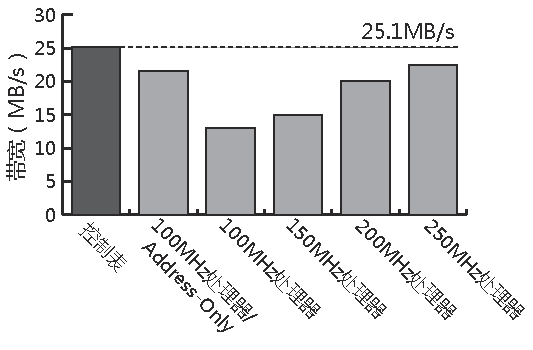
\includegraphics[width=\textwidth]{impl/pard-dp-stream}
  \caption{访存带宽对比}
  \label{fig:pard-dp-stream}
\end{minipage}\hfill
\begin{minipage}{0.48\textwidth}
  \centering
  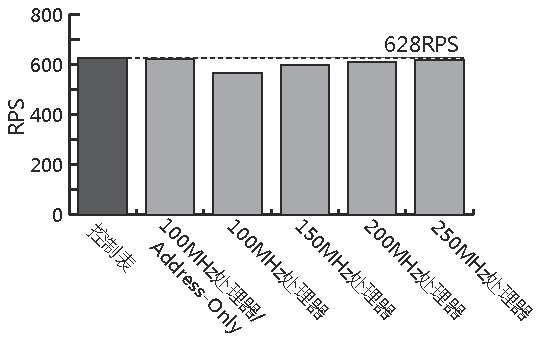
\includegraphics[width=\textwidth]{impl/pard-dp-memcached}
  \caption{memcached性能对比}
  \label{fig:pard-dp-memcached}
\end{minipage}
\end{figure}


\section{资源开销评估}

PARD的资源开销主要体现在三个方面,分别是:
用于标签传播的资源开销、
控制平面的资源开销、
数据平面的资源开销。
本节将分别对这三方面的开销进行评估。

\subsection{标签传播资源开销}

\subsection{控制平面资源开销}

控制平面的资源开销主要体系在表存储、触发逻辑两方面,
使用CAM结构,因此需要消耗大量的LUT和FF资源。具体如表\ref{tab:pard-cp-resource}所示。


\subsection{数据平面资源开销}

可编程数据平面的资源开销主要在处理器逻辑及其使用的scratchpad memory两个方面。
在通过配置精简后,MicroBlaze处理器所占用的资源量大大减少,
其Slice(LUT和FF)占用只有完整配置的50\%左右,
scratchpad memory的容量由固件代码的大小决定,
当前的实现中我们为其保留了32KB的容量,在FPGA中占用了8个RAMB36资源。
原型系统中主要的硬件部件与可编程数据平面占用的FPGA资源如表\ref{tab:pard-dp-resource}所示。
可以看到可编程数据平面在只占用有限的FPGA资源下,为硬件增加了更为灵活的可编程能力。

\begin{table}[htb]
  \centering
  \begin{minipage}[t]{0.9\linewidth}
  \caption{数据平面处理器、共享缓存与内存控制器资源占用情况(xc7vx690t设备)}
  \label{tab:pard-dp-resource}
    \begin{tabular*}{\linewidth}{cccc}
      \toprule[1.5pt]
      \textbf{组件} & \textbf{Slice LUT} & \textbf{Slice Register} & \textbf{Block RAM(RAMB36)} \\
      \midrule[1pt]
      16-way/512KB共享缓存    &  7590       &  5664            &  161               \\
      内存控制器              &  13471      &  10562           &  1                 \\
      完整配置的MicroBlaze核  &  4896       &  8526            &  12                \\
      \hline
      数据平面处理器          &  1433       &  5524            &  8                 \\
      \bottomrule[1.5pt]
    \end{tabular*}\\[2pt]
  \end{minipage}
\end{table}


\section{小结}


\begin{figure}[htb]
  \centering
  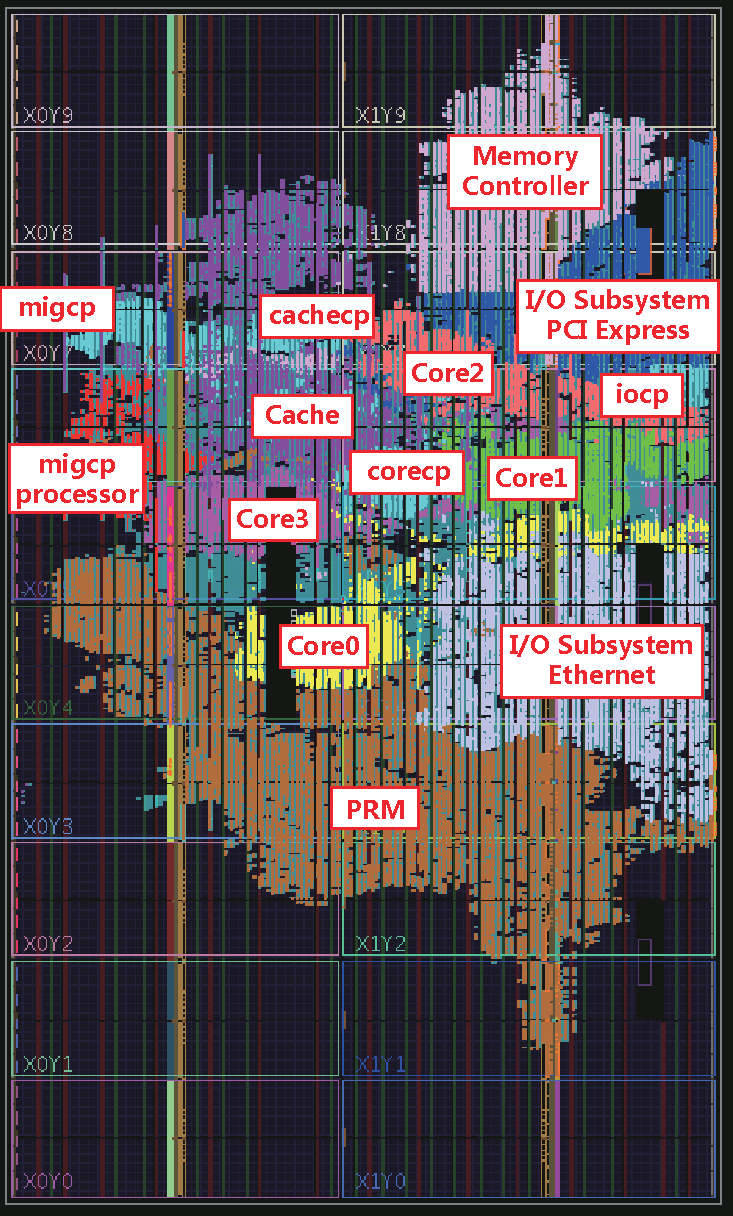
\includegraphics[width=0.8\textwidth]{impl/pard-fpga-routed}
  \caption{PARD原型系统布局布线结果}
  \label{fig:pard-fpga-routed}
\end{figure}
